
% xetex expected
\documentclass[xetex,professionalfont]{beamer}

% we want math
\usepackage{amsmath}

% fixes and extensions to amsmath
\usepackage{mathtools}

% additional math symbols
\usepackage{amssymb}

% good-looking fractions in text via \sfrac
\usepackage{xfrac}

% fix spaces after custom commands (see below for examples)
\usepackage{xspace}

% minted allows for fancy syntax highlighting (requires python with pygments)
% usage:
%   \begin{minted}{python}
%   codeb
%   \end{minted}
\usepackage{minted}

% better looking tables
% usage:
%   begin with a \toprule, write a single row of column headings,
%   then add \midrule and after the columns of data we finish with \bottomrule
% example:
%   \begin{tabular}{llr} \toprule
%   Animal & Description & Price \midrule
%   cat & foo & 10 \\
%   dog & bar & 20 \\ \bottomrule
%   \end{tabular}
% note that good tables generally neither have vertical rules nor double rules
\usepackage{booktabs}

% system font support (requires xetex or luatex)
\usepackage{fontspec}
\setmonofont[Scale=0.7]{Cousine} % part of ttf-chromeos fonts on Arch

% multi-language quotes for babel
\usepackage{csquotes}

% easy way to include copyright information
\usepackage{copyrightbox}

% better bibliographies
\usepackage[backend=biber,style=authoryear]{biblatex}

% language support (english,ngerman)
\usepackage[english]{babel}

% minted screws up line spacings ...
\usepackage{setspace}
\usepackage{enumitem}

% -----------------------------------------------------------------------------

% specify PDF metadata
\hypersetup{pdftitle={CVSP VO - Object Category Recognition},pdfsubject={},pdfauthor={Christopher Pramerdorfer}}

% copyright font style
\makeatletter\renewcommand{\CRB@setcopyrightfont}{\tiny\color{lightgray}}

% add bib file
\addbibresource{literature.bib}

% use tuwcvl beamer theme
\usetheme{tuwcvl}

% add some space between lines
\setstretch{1.4}

% but not for minted environments
\AtBeginEnvironment{minted}{\singlespacing}

% fix itemize

\setlist{nolistsep}
\setitemize{itemsep=-1mm,label=\usebeamerfont*{itemize item}%
  \usebeamercolor[fg]{itemize item}
  \usebeamertemplate{itemize item}}

% -----------------------------------------------------------------------------

% common english abbreviations
\newcommand{\ie}{\mbox{i.e.}\xspace} % i.e.
\newcommand{\eg}{\mbox{e.g.}\xspace} % e.g.

% math - argmin and argmax
\DeclareMathOperator*{\argmin}{arg\,min}
\DeclareMathOperator*{\argmax}{arg\,max}

% shortcuts for number ranges
\newcommand{\NN}{\mathbb{N}}
\newcommand{\ZZ}{\mathbb{Z}}
\newcommand{\QQ}{\mathbb{Q}}
\newcommand{\RR}{\mathbb{R}}

% bold vectors
\renewcommand{\vec}[1]{\ensuremath{\mathbf{#1}}}

% vector shortcuts
\newcommand{\va}{\vec{a}}
\newcommand{\vb}{\vec{b}}
\newcommand{\vc}{\vec{c}}
\newcommand{\ve}{\vec{e}}
\newcommand{\vr}{\vec{r}}
\newcommand{\vs}{\vec{s}}
\newcommand{\vt}{\vec{t}}
\newcommand{\vu}{\vec{u}}
\newcommand{\vv}{\vec{v}}
\newcommand{\vw}{\vec{w}}
\newcommand{\vx}{\vec{x}}
\newcommand{\vy}{\vec{y}}
\newcommand{\vz}{\vec{z}}

\newcommand{\vE}{\vec{E}}
\newcommand{\vF}{\vec{F}}

\newcommand{\bth}{\boldsymbol{\theta}}
\newcommand{\intr}{\boldsymbol{\Lambda}}

% highlight
\newcommand{\highlight}[1]{\textcolor{tuwcvl_inf_red}{\textbf{#1}}}

% make emph red
\let\oldemph\emph
\renewcommand\emph[1]{\textcolor{tuwcvl_inf_red}{#1}}

% -----------------------------------------------------------------------------

\title{Computer Vision Systems Programming VO}
\subtitle{Object Category Recognition}
\author{Christopher Pramerdorfer}
\institute{Computer Vision Lab, Vienna University of Technology}

\begin{document}

% -----------------------------------------------------------------------------

\begin{frame}
\maketitle
\end{frame}

% -----------------------------------------------------------------------------

\begin{frame}
\frametitle{Topics}

Scene classification using the bag of words model \\
Fast face detection using boosted Haar features \\
Convolutional neural networks for large-scale problems

\bigskip
\begin{center}
    \copyrightbox[b]
    {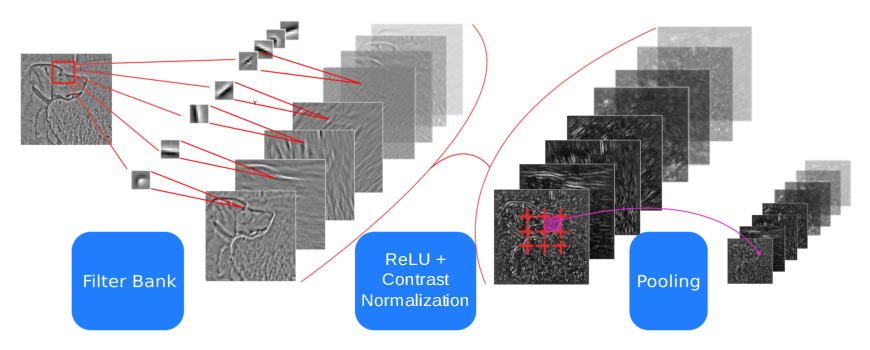
\includegraphics[width=7cm]{figures/cnp-layers.png}}
    {\centering Image adaoted from \cite{kavukcuoglu2011}}
\end{center}

\end{frame}

% -----------------------------------------------------------------------------

\begin{frame}
\frametitle{Scene Classification}

We want to distinguish between $c$ scene categories
\begin{itemize}
    \item So $w\in\{0,\dots,c-1\}$ (classification problem)
\end{itemize}

\medskip
\begin{center}
    \copyrightbox[b]
    {
\begin{tikzpicture}
    \node[anchor=south west,inner sep=0] (image) at (0,0) {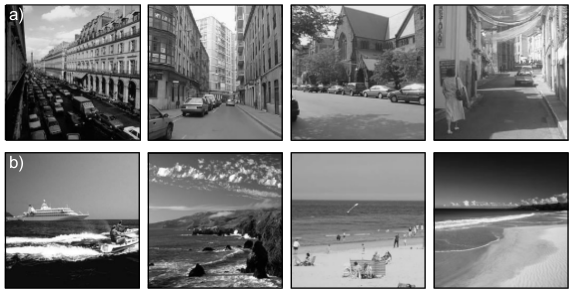
\includegraphics[width=7.75cm]{figures/scene-categories.jpg}};
    \begin{scope}[x={(image.south east)},y={(image.north west)}]
        \node[red] at (-0.13,0.25) {Sea Scenes};
        \node[red] at (-0.15,0.75) {Street Scenes};
    \end{scope}
\end{tikzpicture}
    }
    {\centering Image adapted from \cite{prince12}}
\end{center}

\end{frame}

% -----------------------------------------------------------------------------

\begin{frame}
\frametitle{Scene Classification}
\framesubtitle{Bag of Visual Words}

We represent an image as a collection of \emph{visual words} % this comes from document retrieval - a text consists of words, an image of visual words, so we represent an image by the distribution of its visual words
\begin{itemize}
    \item Images can be compared based on visual word distribution
\end{itemize}

\medskip
\begin{center}
    \copyrightbox[b]
    {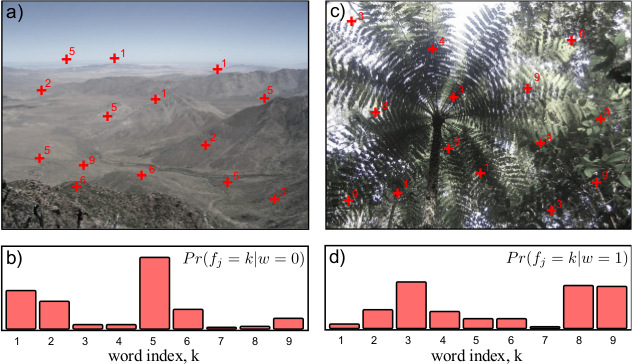
\includegraphics[width=7cm]{figures/visual-words.jpg}} % we see that the visual word representations of these images differ, so they are not of the same class
    {\centering Image from \cite{prince12}}
\end{center}

\end{frame}

% -----------------------------------------------------------------------------

\begin{frame}
\frametitle{Scene Classification}
\framesubtitle{Bag of Visual Words}

Visual words are learned from an image collection
\begin{itemize}
    \item Compute (SIFT) keypoints and descriptors for all images
    \item Cluster descriptors into $k$ clusters using $k$-means % this is the standard method, can use other clustering methods as well
    \item $k$ cluster means represent visual words
\end{itemize}

\medskip
\begin{center}
    \copyrightbox[b]
    {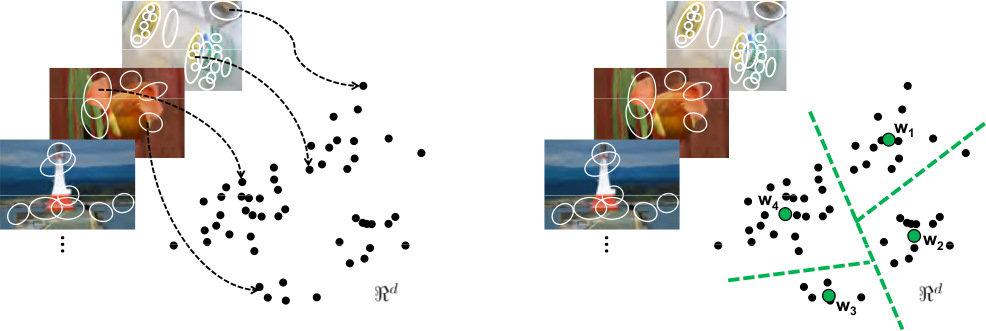
\includegraphics[width=8.5cm]{figures/visual-word-construction.jpg}}
    {\centering Image from \cite{grauman2011}}
\end{center}

\end{frame}

% -----------------------------------------------------------------------------

\begin{frame}
\frametitle{Scene Classification}
\framesubtitle{Bag of Visual Words}

Visual word distribution $\vx\in\NN^k$ of image obtained by
\begin{itemize}
    \item Computing keypoints and descriptors
    \item Assigning each feature to closest visual word % this is again the simplest approach, better performance can be achieved using fuzzy assignment
    \item Summing up the assignment counts for each visual word % and normalizing them of course
\end{itemize}

\medskip
\begin{center}
    \copyrightbox[b]
    {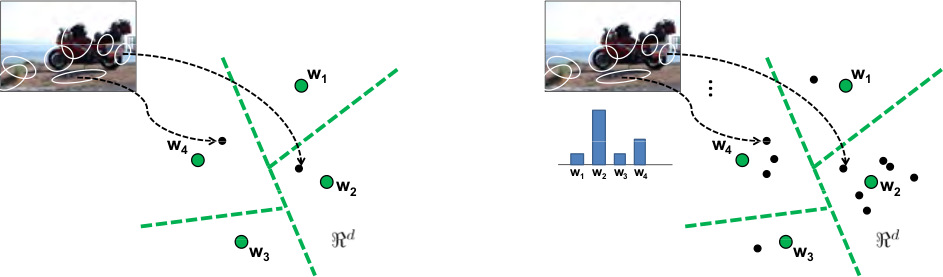
\includegraphics[width=8.5cm]{figures/visual-word-generation.jpg}}
    {\centering Image from \cite{grauman2011}}
\end{center}

\end{frame}

% -----------------------------------------------------------------------------

\begin{frame}
\frametitle{Scene Classification}
\framesubtitle{Bag of Visual Words}

This image representation is called \emph{bag of (visual) words}

\bigskip
Now that we have $\vx$ we can select and learn a suitable model
\begin{itemize}
    \item SVMs are often used in the literature
    \item For a probabilistic alternative see \cite{prince12}
\end{itemize}

\end{frame}

% -----------------------------------------------------------------------------

\begin{frame}
\frametitle{Scene Classification}
\framesubtitle{Bag of Visual Words -- Remarks}

Many improvements to this model exist
\begin{itemize}
    \item Better clustering schemes
    \item Fuzzy assignment to visual words
    \item Spatial information (constellation model)
\end{itemize}

\bigskip
Popular and can work well, but no longer state of the art % for this reason, this was quite short, basically in order to make the differences to deep learning clearer

\end{frame}

% -----------------------------------------------------------------------------

{
\setbeamertemplate{footline}{}
\begin{frame}

\begin{tikzpicture}[remember picture,overlay]
\fill[white] (current page.north west) rectangle (current page.south east);
\end{tikzpicture}

\end{frame}
}

% -----------------------------------------------------------------------------

\begin{frame}
\frametitle{Face Detection}

\begin{center}
    \copyrightbox[b]
    {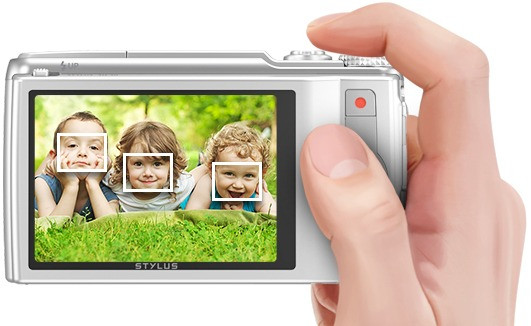
\includegraphics[width=7cm]{figures/camera-faces.jpg}}
    {\centering Image from \url{olympus-europa.com}}
\end{center}

\end{frame}

% -----------------------------------------------------------------------------

\begin{frame}
\frametitle{Face Detection}

Many applications
\begin{itemize}
    \item Smart cameras (autofocus on faces)
    \item Security (preprocessing step to face recognition)
    \item Augmented reality
\end{itemize}

\end{frame}

% -----------------------------------------------------------------------------

\begin{frame}
\frametitle{Face Detection}

We don't know where the faces are so we % could be 0, could be 10, arbitrary positions
\begin{itemize}
    \item Slide a fixed-size window over the image
    \item Compute $\Pr(w|\vx)$ for each window ($w=1$ if face, 0 if not)
\end{itemize}

\medskip
\begin{center}
\begin{tikzpicture}
\node [inner sep=0pt,above right]{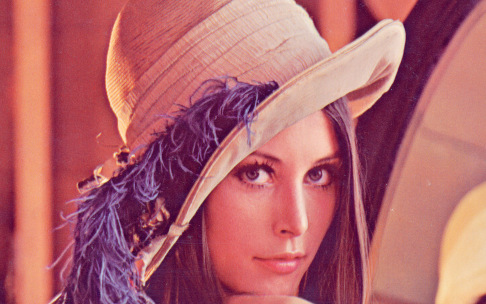
\includegraphics[width=5cm]{figures/lena.jpg}};;
\draw[thick,green,opacity=0.2] (1.6,0.25) rectangle (3.6,2.25);
\draw[thick,green,opacity=0.4] (1.7,0.25) rectangle (3.7,2.25);
\draw[thick,green,opacity=0.6] (1.8,0.25) rectangle (3.8,2.25);
\draw[thick,green,opacity=0.8] (1.9,0.25) rectangle (3.9,2.25);
\draw[thick,green] (2,0.25) rectangle (4,2.25);
\end{tikzpicture}
\end{center}

\end{frame}

% -----------------------------------------------------------------------------

\begin{frame}
\frametitle{Face Detection}

Many windows, so computing $\vx$ and $\Pr(w|\vx)$ must be fast \\
We focus on the popular method from \cite{viola2001}

\end{frame}

% -----------------------------------------------------------------------------

\setstretch{1}
\renewcommand\emph[1]{\oldemph{#1}}

\begin{frame}[allowframebreaks=0.9]
\frametitle{Bibliography}

\printbibliography

\end{frame}

\end{document}
